\documentclass[tikz,border=3pt]{standalone}
\usepackage{pgfplots}
\pgfplotsset{compat=1.15}
\usepackage{mathrsfs}
\usetikzlibrary{arrows}
\usetikzlibrary{patterns}
\usepackage{graphicx}

\begin{document}

	% The x=1cm, y=1cm units are used again, and all coordinates are 10x larger 
	% than the previous 1mm code, achieving the final 10x scale.
	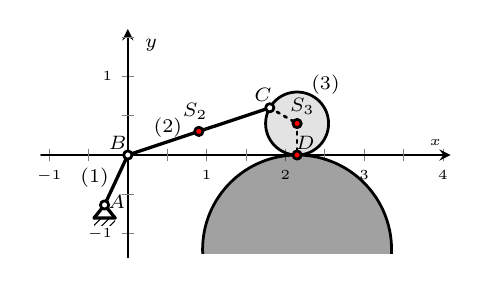
\begin{tikzpicture}[line cap=round,line join=round,>=triangle 45,x=1cm,y=1cm, font=\scriptsize] 
		\begin{axis}[
			axis lines=middle,
			axis line style={thick},
			x=1cm,y=1cm, 
			% Axis limits are the previous * 10
			xmin=-1.1,
			xmax=4.1,
			ymin=-1.3,
			ymax=1.6,
			xlabel={\tiny $x$},
			ylabel={\ $y$},
			xtick={-3,-2,...,4},
			ytick={-3,-2,...,1},
			extra x ticks={-3.5,-2.5,...,3.5},
			extra x tick labels={},
			extra y ticks={-3.5,-2.5,...,1.5},
			extra y tick labels={},
			tick label style={font=\tiny},
			]

			\clip(-1.236748841576818,-1.254613518011875) rectangle (7.299066435311561,1.324851060429165);
			
			\draw [line width=1pt,fill=black,fill opacity=0.37] (2.1491857992457702,-1.2) circle (1.2cm); 

			\draw [line width=1pt,fill=black,fill opacity=0.11] (2.1491857992457702,0.4) circle (0.4cm); 

			\draw [line width=1.2pt] (-0.29583278321848965,-0.634415450925655)-- (0,0);
			\draw [line width=1.2pt] (0,0)-- (1.8027756377319948,0.6);
			
			\draw [line width=1.2pt] (-0.29583278321848965,-0.634415450925655)-- (-0.4294666109065957,-0.8009221549646055);
			\draw [line width=1.2pt] (-0.4294666109065957,-0.8009221549646055)-- (-0.1614851413704704,-0.800346742964898);
			\draw [line width=1.2pt] (-0.1614851413704704,-0.800346742964898)-- (-0.29583278321848965,-0.634415450925655);
			
			\draw[pattern=north east lines, pattern color=black, draw=none]
			(axis cs:-0.4294666109065957,-0.800346742964898) rectangle (axis cs:-0.1614851413704704,-0.900346742964898);
			
			\draw [line width=1pt,dash pattern=on 1pt off 2pt] (1.8027756377319948,0.6)-- (2.1491857992457702,0.4);
			\draw [line width=1pt,dash pattern=on 1pt off 2pt] (2.1491857992457702,0.4)-- (2.1491857992457702,0);
			\begin{normalsize}
				\draw [fill=white, line width=1pt] (0,0) circle (1.5pt);
				\draw[color=black] (-0.12787356851102264,0.1483946834953474) node {$B$};
				
				\draw [fill=white, line width=1pt] (-0.29583278321848965,-0.634415450925655) circle (1.5pt);
				\draw[color=black] (-0.14078924975748524,-0.5903826719406648) node {$A$};
				
				\draw [fill=white, line width=1pt] (1.8027756377319948,0.6) circle (1.5pt);
				\draw[color=black] (1.717882884580667,0.7630077775135424) node {$C$};
				
				\draw [fill=red, line width=1pt] (2.1491857992457702,0) circle (1.5pt);
				\draw[color=black] (2.252123504110155,0.1597700442826748) node {$D$};
				
				\draw [fill=red, line width=1pt] (0.9013878188659974,0.3) circle (1.5pt);
				\draw[color=black] (0.854941267726836,0.5519285331032532) node {$S_2$};
				
				\draw [fill=red, line width=1pt] (2.1491857992457702,0.4) circle (1.5pt);
				\draw[color=black] (2.2145399302519367,0.6208874677487989) node {$S_{3}$};
				
				\draw[color=black] (-0.42253708503352093,-0.2923884445379036) node {(1)};
				\draw[color=black] (0.50728133575694716,0.3522246494802914) node {(2)};
				\draw[color=black] (2.510337489778284,0.8871720389313595) node {(3)};
			\end{normalsize}
		\end{axis}
	\end{tikzpicture}
\end{document}